\documentclass[vecarrow]{svproc}
% % RECOMMENDED  % to typesetURLs, URIs, and DOIs
\usepackage{url}
\def\UrlFont{\rmfamily}

\usepackage{listings}
\usepackage{color}
\definecolor{dkgreen}{rgb}{0,0.6,0}
\definecolor{gray}{rgb}{0.5,0.5,0.5}
\definecolor{mauve}{rgb}{0.58,0,0.82}
\lstset{frame=tb,
 aboveskip=3mm, belowskip=3mm,
showstringspaces=false, columns=flexible,
basicstyle={\small\ttfamily}, numbers=none,
numberstyle=\tiny\color{gray}, keywordstyle=\color{blue},
commentstyle=\color{dkgreen},
stringstyle=\color{mauve}, breaklines=true,
breakatwhitespace=true, tabsize=3 }

\usepackage{graphicx}

\usepackage{booktabs}

\usepackage{rotating}

\usepackage{pdflscape}

%\usepackage{amsmath}

\begin{document}
\mainmatter % start of a contribution %

\title{Learning tensorflow} %

\titlerunning{Learning tensorflow}
% abbreviated title (for running head)
% also used for the TOC unless
% \toctitle is used %
\author{Mohd Zamri Murah} %
%\authorrunning{Ivar Ekeland et al.} % abbreviated author list (for running head)
% list of authors for the TOC (use if author list has to be modified)
%\tocauthor{Ivar Ekeland, Roger Temam, Jeffrey Dean, David
 \institute{Center for Artificial Intelligence
Technology\\ Fakulti Teknologi Sains
Maklumat\\ Universiti Kebangsaan Malaysia\\
\email{zamri@ukm.edu.my}}

\maketitle % typeset the title of the contribution

\begin{abstract}

Tensorflow is an open-source
deep learning library developed by Google.
It has been used in many areas such as image recognition, text
to speech engine, pattern recognition and
big data. This note provide an introductory concepts for
computation using tensorflow.

\keywords{deep learning}

\end{abstract} %

\section{Introduction}

Tensorflow is an open-source deep learning library
developed by Google\cite{abadi2015tensorflow}. It is based on
two basic ideas; computational graph and
tensor.

A basic computational graph is shown in
figure~\ref{fig:1}. The figure illustrates the two
elements of computational graph; nodes and edges. Nodes
typically drawn as circles to represent some sort
of computation or action being done on data. Edges are the
actual values that get passed to and from
nodes, and are typically drawn as arrows. Thus, in
figure~\ref{fig:1}, we have a node for computation
$add$  and edge $1$ and edge $2$ into the node $add$ and,
edge $3$ as edge output from the node
$add$.

\begin{figure}
% https://en.wikibooks.org/wiki/LaTeX/Importing_Graphics
% Use the relevant command to insert your figure file.
% For example, with the graphicx package use
\centering{\fbox{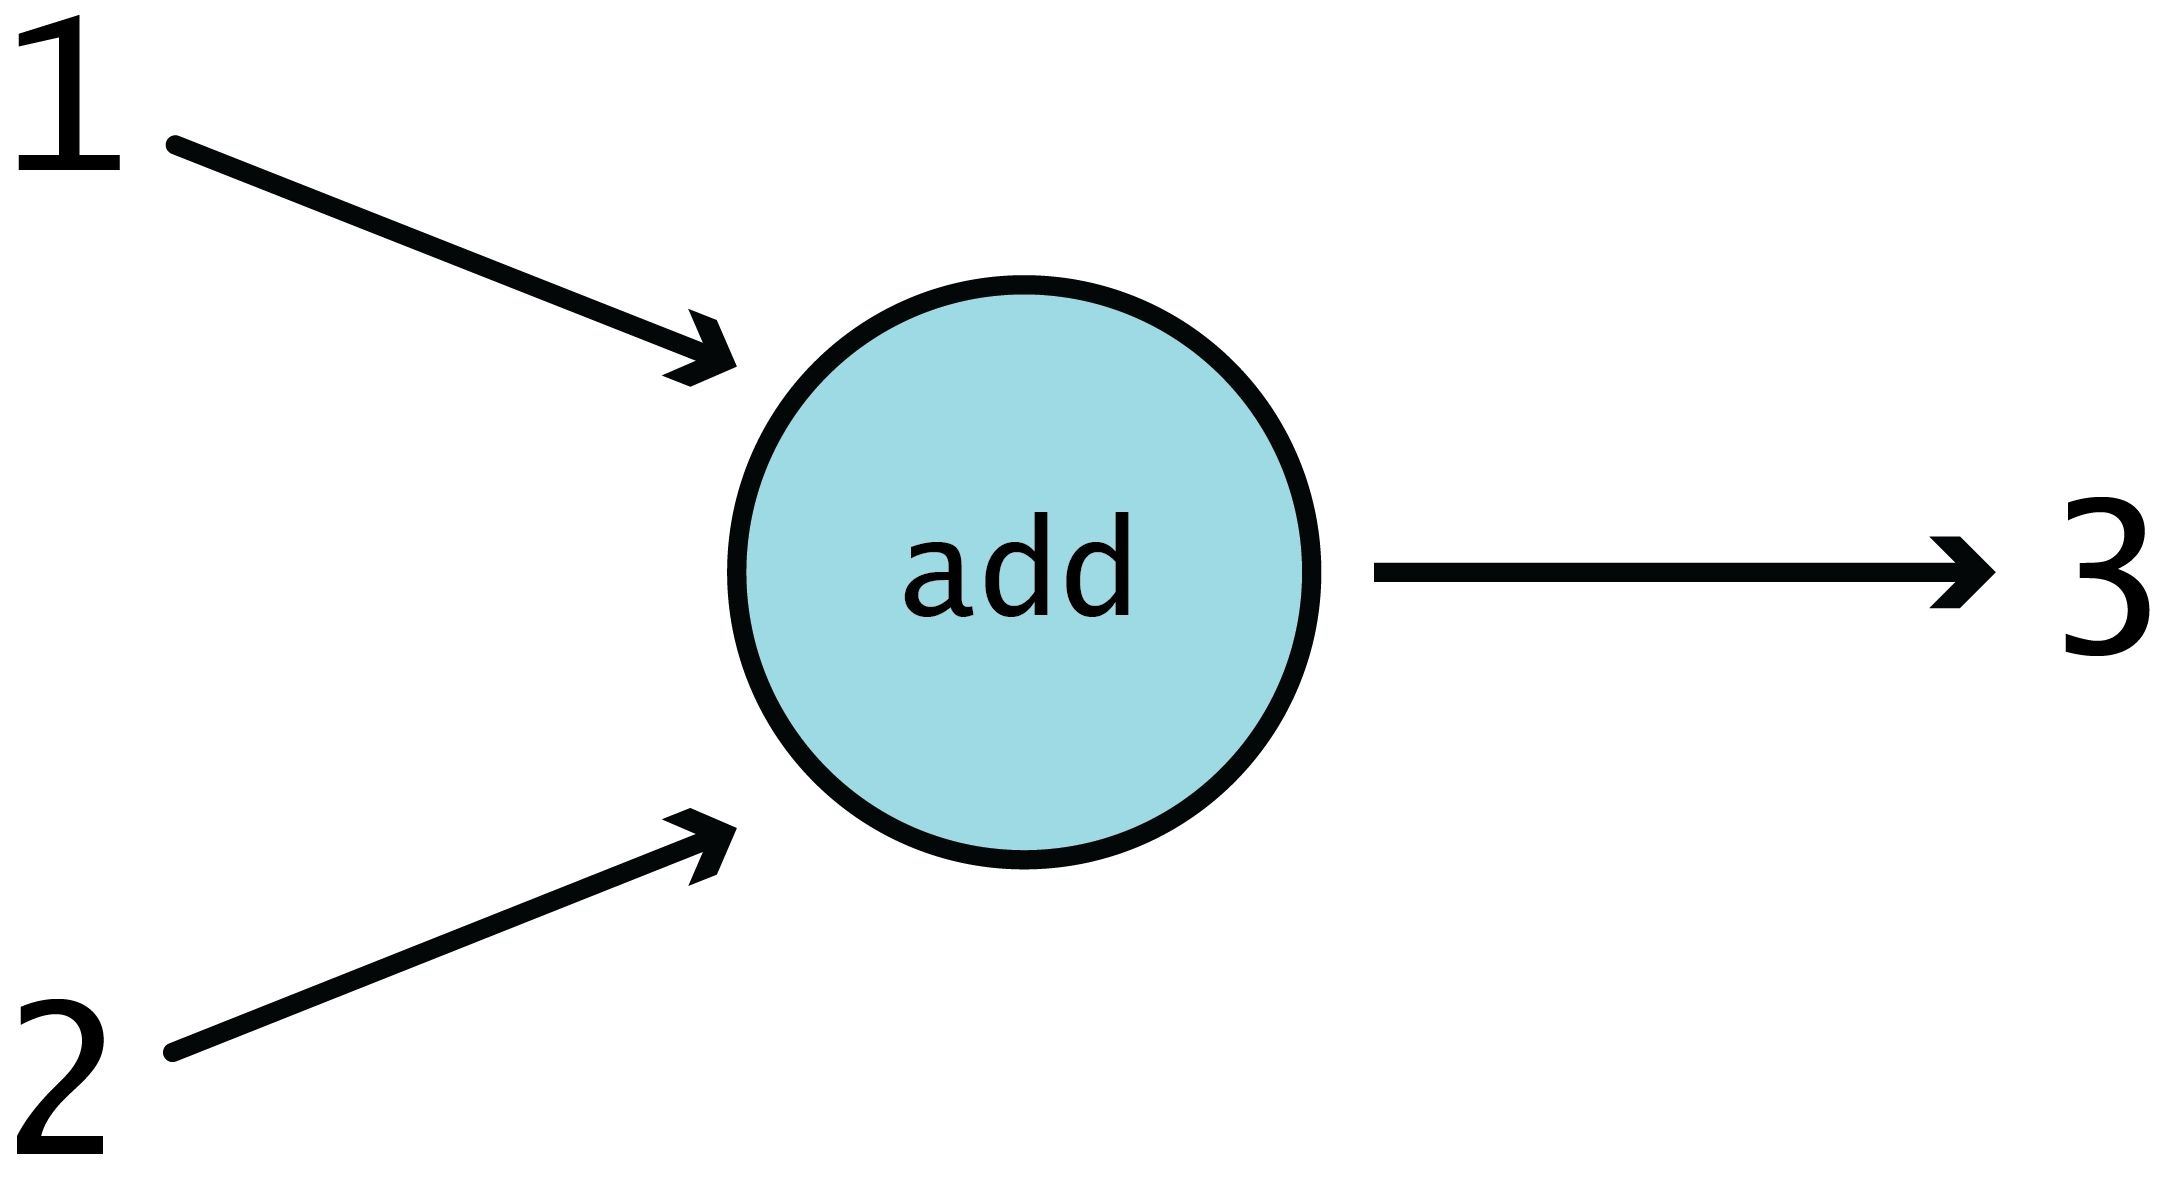
\includegraphics[scale=.10]{basic_node.png}}} %
\caption{A basic computational graph with node and edge.}
\label{fig:1}
% Give a unique label
\end{figure}

In figure~\ref{fig:2}, we have a more complex computation. In figure~\ref{fig:2}, we have nodes $input$, $input$,
$add$,$mult$ and $add$. In total, we have 5 nodes. Also, we have 9 edges; $5,3,5,5,3,3,15,8,23$. Succintly, we could write the model as; $ N=\{input, add,mult, add\}$ and $E=\{5,3,5,5,3,3,15,8,23\}$.

\begin{figure}
% https://en.wikibooks.org/wiki/LaTeX/Importing_Graphics
% Use the relevant command to insert your figure file.
% For example, with the graphicx package use
\centering{\fbox{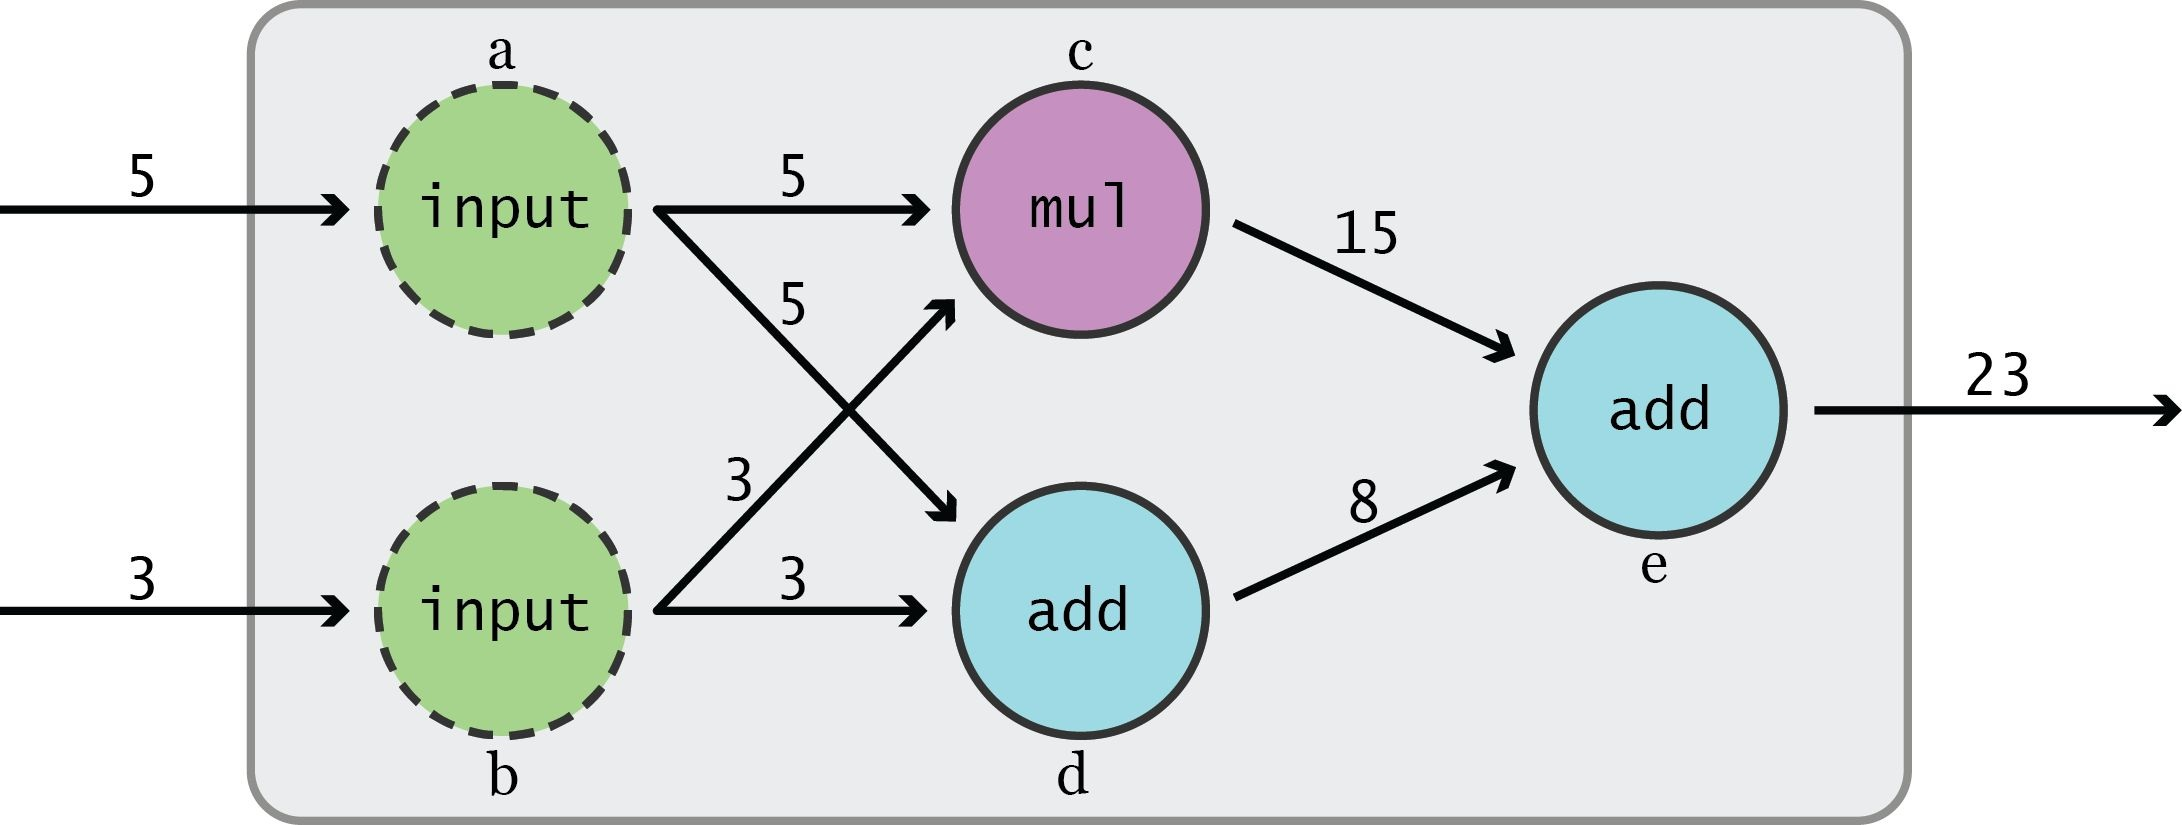
\includegraphics[scale=.10]{node_2.png}}} %
\caption{A more complex computational graph with nodes and edges.}
\label{fig:2}
% Give a unique label
\end{figure}

We can also have a more complicated model as figure~\ref{fig:3}.

\begin{figure}
% https://en.wikibooks.org/wiki/LaTeX/Importing_Graphics
% Use the relevant command to insert your figure file.
% For example, with the graphicx package use
\centering{\fbox{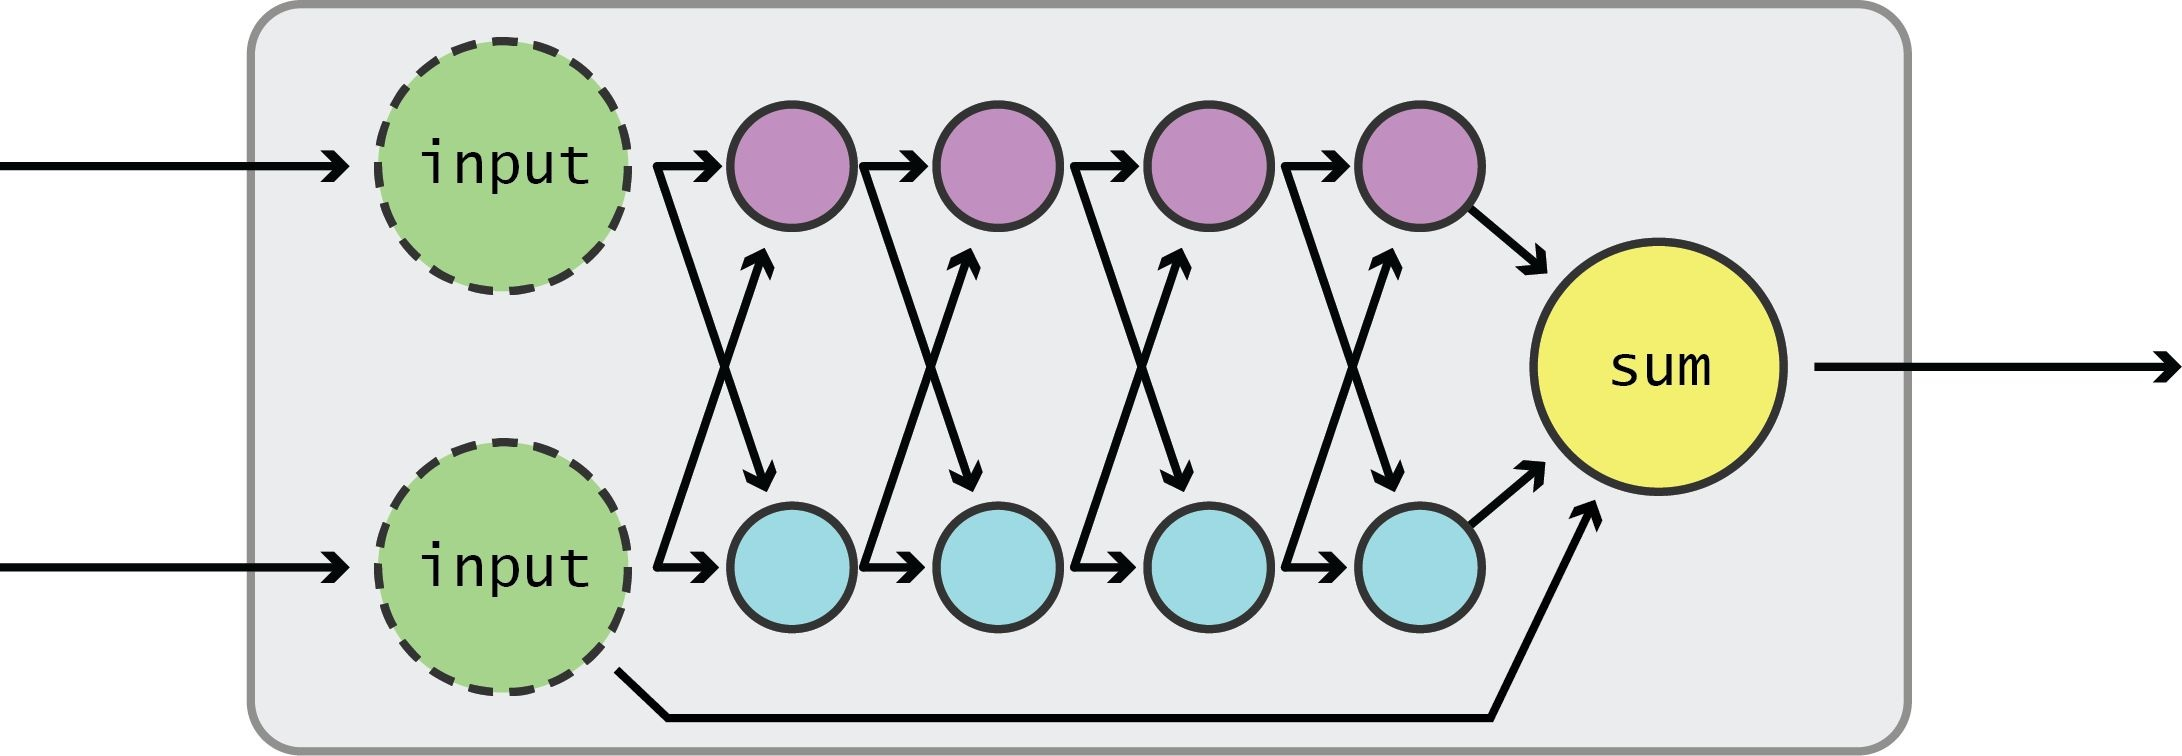
\includegraphics[scale=.10]{node_3.png}}} %
\caption{A edge can link to any node.}
\label{fig:3}
% Give a unique label
\end{figure}


\section{Computational graph}

Tensorflow computation is based on computational graph. In order to model in tensorflow, we need to;
\begin{enumerate}
\item define model in computational graph
\item run model
\end{enumerate}

In listing~\ref{list1}, we provide the code for a tensor model based on our previous discussion.

\renewcommand{\thelstlisting}{\arabic{lstlisting}}

\begin{lstlisting}[language=Python,
caption={an example of tensorflow model},label={list1}]
import	tensorflow	as	tf
a =	tf.constant(5, name="input_a")
b =	tf.constant(3, name="input_b")
c =	tf.mul(a,b, name="mul_c")
d =	tf.add(a,b, name="add_d")
e = tf.add(c,d, name="add_e")
sess = tf.Session()
output = sess.run(e)
writer = tf.train.SummaryWriter('./my_graph', sess.graph)
writer.close()
sess.close()
\end{lstlisting}

If we run tensorboard, we have the figure~\ref{fig:4}.
% tensorboard	--logdir="my_graph"

\begin{figure}
% https://en.wikibooks.org/wiki/LaTeX/Importing_Graphics
% Use the relevant command to insert your figure file.
% For example, with the graphicx package use
\centering{\fbox{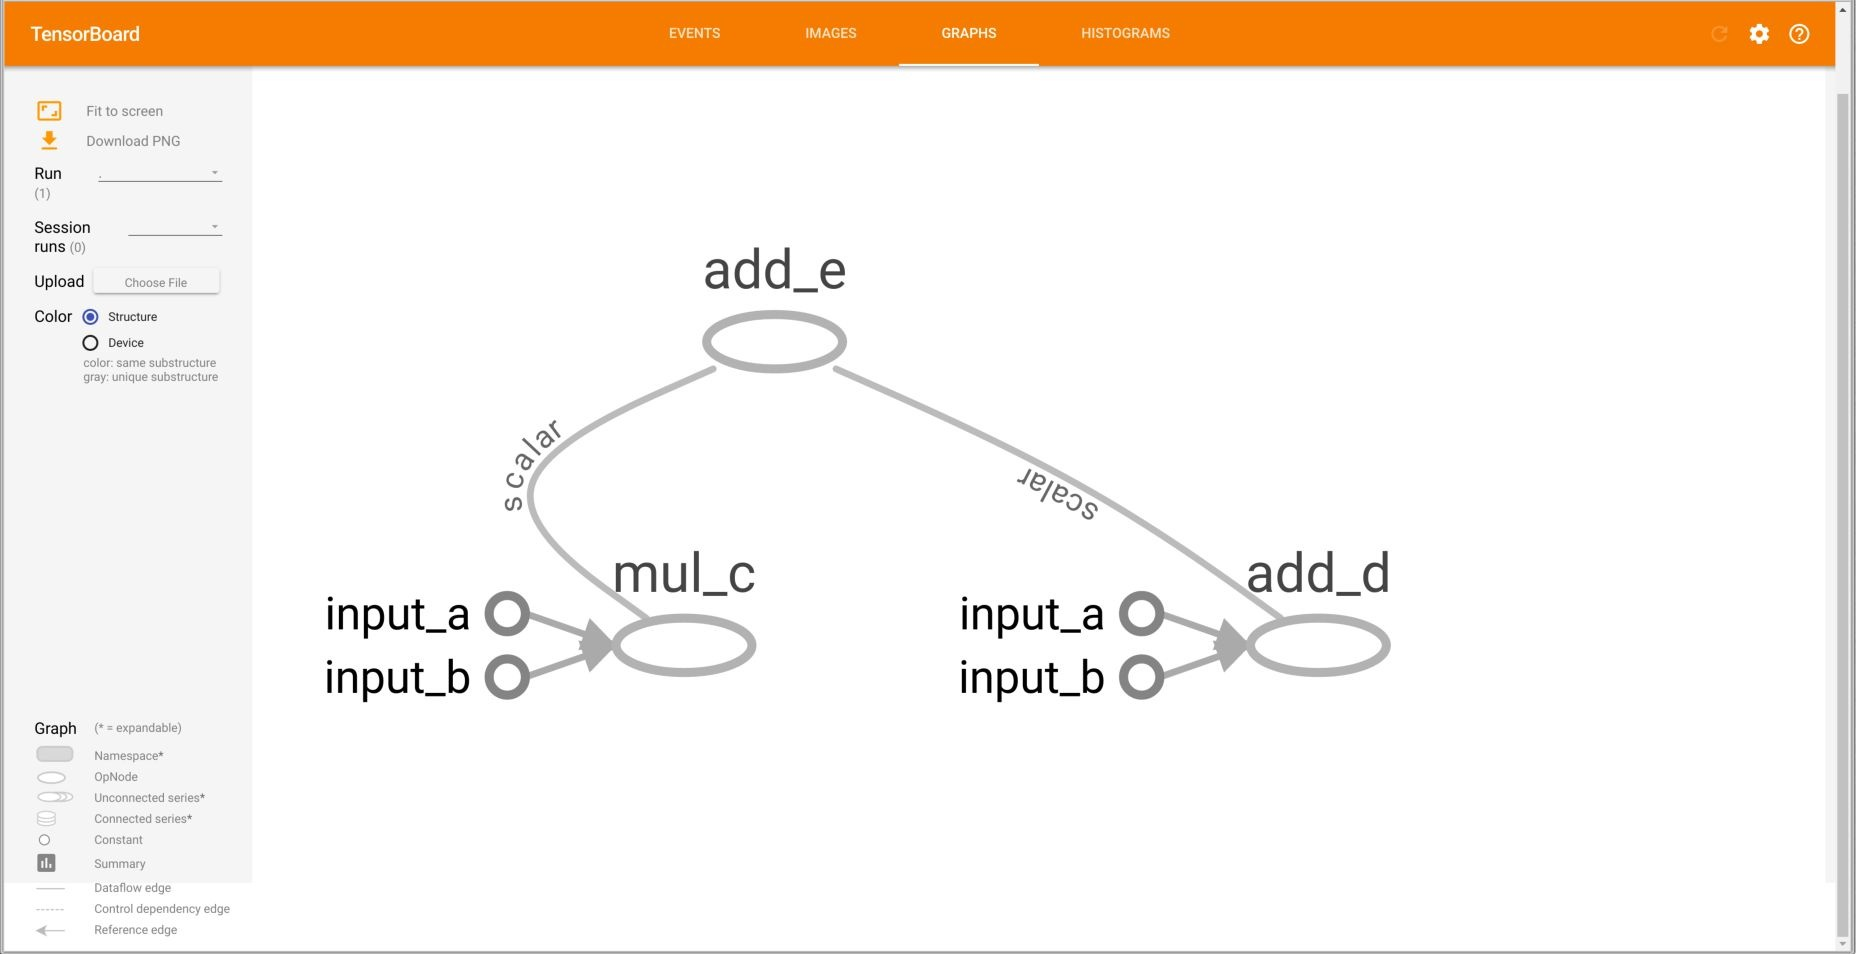
\includegraphics[scale=.10]{node_4.png}}} %
\caption{A graphical view of the tensorflow model using tensorboard.}
\label{fig:4}
% Give a unique label
\end{figure}

\section{Tensor}

Tensorflow data model is based on tensor. Tensor is an $n$-dimensional abstraction of matrices. We have
scalar $\eta=[5]$ equivalent to 0-D tensor, a vector $\vec{v}=[5, 3]$ equivalent to 1-D tensor and a matrix
$A_{m,n}$ is a 2-D tensor\cite{bowen2008introduction}\cite{kolecki2002introduction}.

Two vectors $\vec{v}$ and $\vec{w}$ can be combined via inner product to form a new scalar $\eta$. Two
vectors $\vec{v}$ and $\vec{w}$ can be combined via cross product to form a new vector $\vec{z}$. Thus we
have the following generalization;
\begin{enumerate}
\item $\eta$ scalar. tensor of rank $0$ with $3^0=1$ component. magnitude only.
\item $vec{v}$ vector. tensor of rank $1$ with $3^1=3$ components. magnitude and one direction.
\item $A$ dyad. tensor of rank $2$ with $3^2=9$ components. magnitude and 2 directions.
\end{enumerate}

Quantities with no sense of direction are scalars $\eta$, these are defined as only real numbers in any system of units such as temperature. Scalr have $1 = 3^0$ element. The vectors $\vec{v}$ on the other hand are associated with direction, force for example. The number of elements are $3 = 3^1$. The second order tensor is a quantity with which two directions seem to be associated. The stress acting on an element of fluid in a 3D Cartesian system acts on planes $xx$, $yy$, $zz$, $xy$, $zx$ and so on a total of $9 = 3^2$ elements define the stress system of the element. Strain rate tensor is another example.

\section{Model in tensor}

In figure~\ref{fig:5}, we have the same model in tensor notation.

\begin{figure}
% https://en.wikibooks.org/wiki/LaTeX/Importing_Graphics
% Use the relevant command to insert your figure file.
% For example, with the graphicx package use
\centering{\fbox{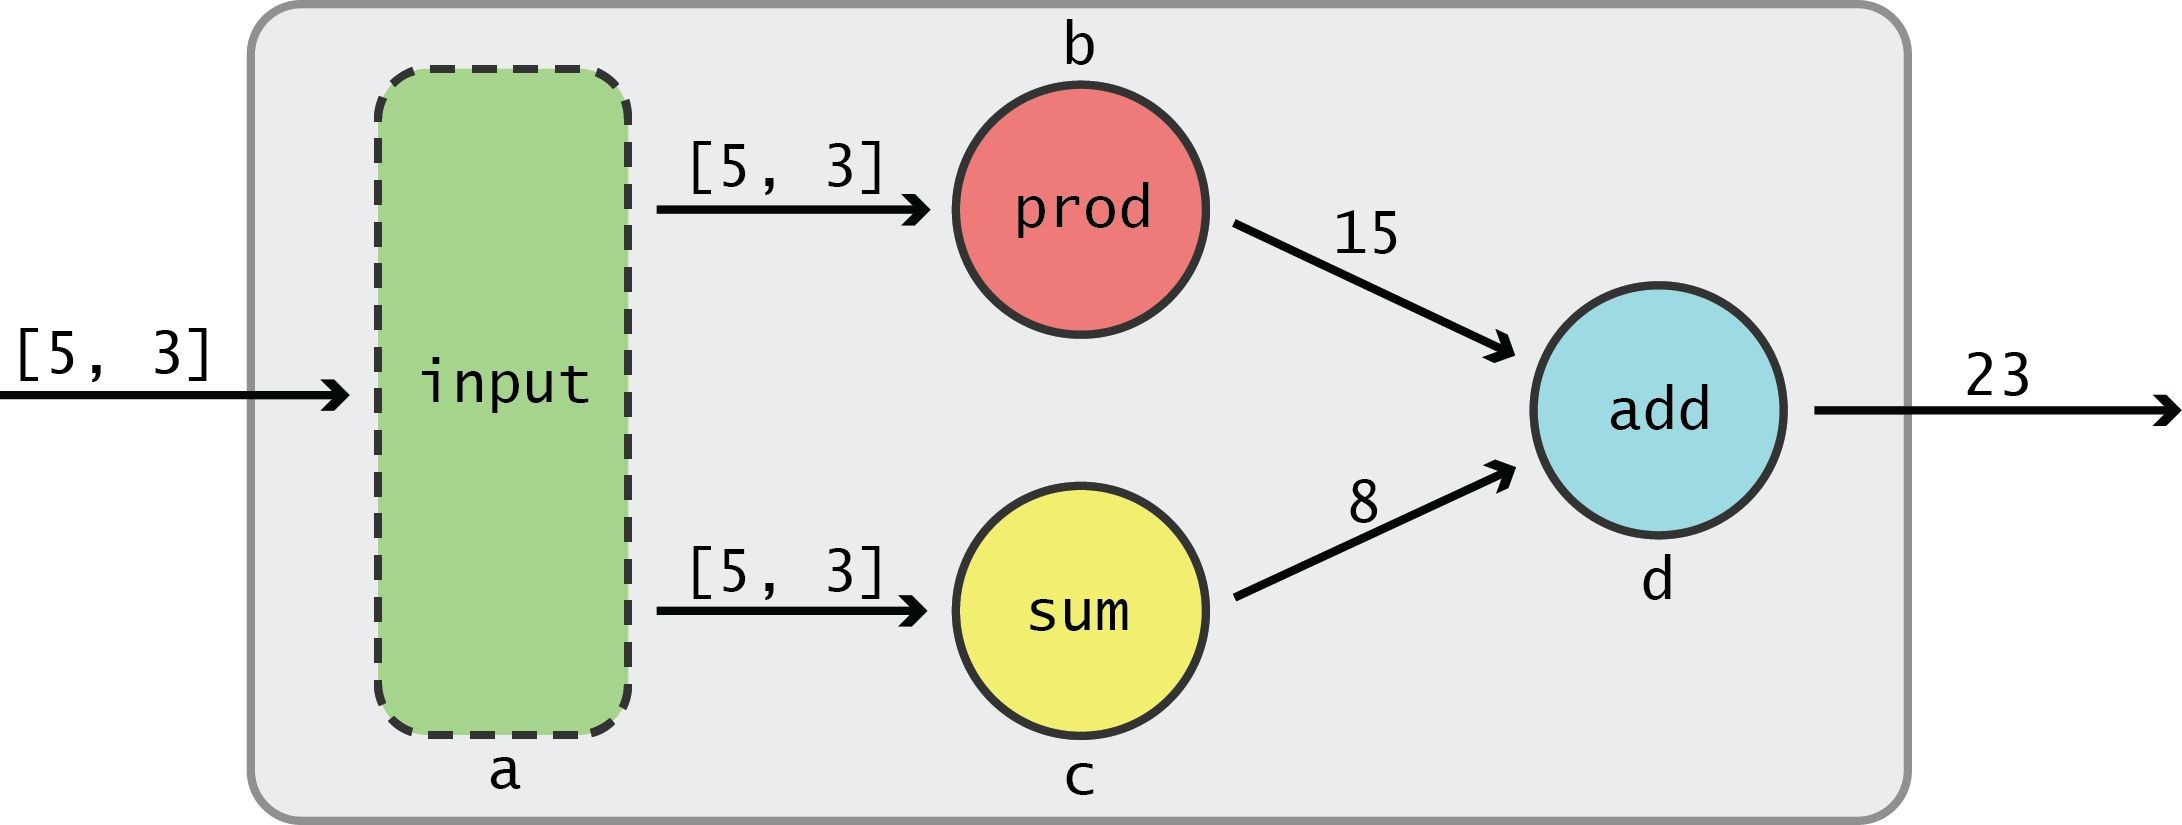
\includegraphics[scale=.10]{node_5.png}}} %
\caption{A graphical view of the tensorflow model using tensorboard.}
\label{fig:5}
% Give a unique label
\end{figure}

\begin{lstlisting}[language=Python,
caption={model in tensor},label={list2}]
import tensorflow as tf
a = tf.constant([5, 3, 9], name="input_a")
b = tf.reduce_prod(a, name="prod_b")
c = tf.reduce_sum(a, name="sum_c")
d = tf.add(b, c, name="add_d")

sess = tf.Session()
sess.run(d)

print(sess.run(d))
output = sess.run(d)
\end{lstlisting}

We could examine the shape of a tensor using $tf.shape$.
\begin{lstlisting}[language=Python,
caption={shape of tensor},label={list3}]
tf.shape(a) # <tf.Tensor 'Shape:0' shape=(1,) dtype=int32>
tf.shape(b) # <tf.Tensor 'Shape_1:0' shape=(0,) dtype=int32>
tf.shape(c) # <tf.Tensor 'Shape_2:0' shape=(0,) dtype=int32>
tf.shape(d) # <tf.Tensor 'Shape_3:0' shape=(0,) dtype=int32>
\end{lstlisting}
%\cite{techreport}.

Tensors	are	just	a	superset	of	matrices!.

\section{Tensors operations}

Nodes in tensorflow are operations on tensors. Nodes perform operation on or with tensor objects, and output tensors objects such as scalar or another tensor. These outputs can be use as input by other nodes in the computational graph. An example of tensor operation is shown in listing~\ref{list4}.

\begin{lstlisting}[language=Python,
caption={operations on tensors},label={list4}]
#Initialize	some	tensors	to	use	in	computation
a = np.array([2,	3],	dtype=np.int32) # tensor a
b =	np.array([4,	5],	dtype=np.int32) # tensor b
#Use tf.add() to initialize an "add" Operation
#The variable `c'	 will	be a	handle to the Tensor output of this	Op
c = tf.add(a,	b)
\end{lstlisting}

\section{Using variables in tensor models}

Variables in tensor models are called \textit{placeholders}. have their values specified when created.

\begin{lstlisting}[language=Python,
caption={use placeholders in tensor},label={list5}]
import tensorflow as tf
import numpy as np
# Creates a placeholder vector of length 2 with data type int32
a = tf.placeholder(tf.int32, shape = [2],name = "my_input")
# Use the placeholder as if it were any other Tensor object
b = tf.reduce_prod(a, name = "prod_b")
c = tf.reduce_sum(a, name = "sum_c")
# Finish off the graph
d = tf.add(b, c, name = "add_d")

#Open a TensorFlow Session
sess = tf.Session()

#Create a dictionary to pass into`feed_dict`
#Key: `a`, the handle to the placeholder output Tensor
#Value: A vector with value[5, 3] and int32 data type
input_dict = { a: np.array([5, 3], dtype = np.int32)}
#Fetch the value of `d`, feeding the values of `input_vector` into `a`
sess.run(d, feed_dict = input_dict)
\end{lstlisting}

Tensors (e.g $a, b , c., d$ in above model)  and $operation$ (e.g node such
$add, mult, reduce_prod$)
objects are immutable ( cannot be changed). $Variables$ objects contain
mutable tensor values that are persistent across sessions.

\begin{lstlisting}[language=Python,
caption={use placeholders in tensor},label={list6}]
import tensorflow as tf
#Pass in a starting value of three for the variable
my_var = tf.Variable(3, name="my_variable")

a = tf.add(5,	my_var)
b =	tf.mul(8,	my_var)
\end{lstlisting}

The	initial value of Variables will often be large tensors of zeros, ones,	or random
values.

\begin{lstlisting}[language=Python,
caption={use placeholders in tensor},label={list7}]
#2x2 matrix	of zeros
zeros = tf.zeros([2,	2])
# vector	 of length 6 of ones
ones = tf.ones([6])
#3x3x3	Tensor of random	uniform	 values between 0 and 10
uniform = tf.random_uniform([3, 3, 3], minval=0, maxval=10)
#3x3x3	Tensor of normally distributed	numbers; mean 0 and standard deviation 2
normal = tf.random_normal([3, 3, 3], mean=0.0,	stddev=2.0)

sess = tf.Session()
sess.run([zeros,ones, uniform, normal])

# proper way to initialize
#init = tf.initialize_all_variables()
#sess = tf.Session()
#sess.run(init)
\end{lstlisting}

\section{Machine learning in tensor}

Supervised learning concerns with inference models where we have input data dan output results. The objective is to find inference models with the minimun loss functions. This is done through training. The inference models can be used for predictions of new input data. The basic training loop is given on figure~\ref{fig:6}.

\begin{figure}
% https://en.wikibooks.org/wiki/LaTeX/Importing_Graphics
% Use the relevant command to insert your figure file.
% For example, with the graphicx package use
\centering{\fbox{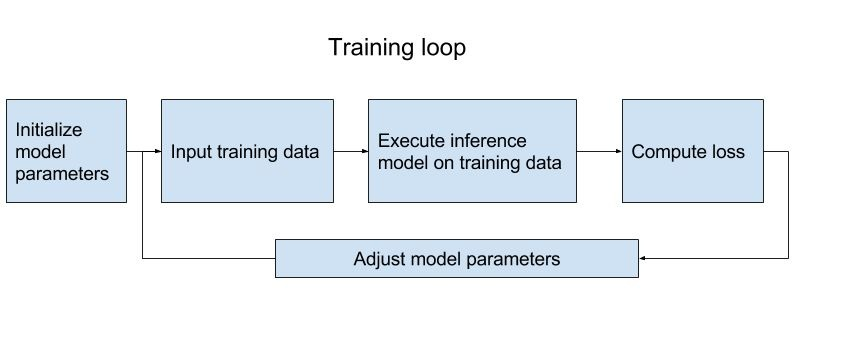
\includegraphics[scale=.40]{training_loop.png}}} %
\caption{A basic training loop.}
\label{fig:6}
% Give a unique label
\end{figure}

\section{Linear regression in tensor}

In linear regression, we have the standard simple linear regression equation as
$ y = ax + b $ or in tensor format we have $ Y = XW^t + b$ where $W$ is weight and
$b$ is bias.

The $L2$ norm loss function is defined as $ L_2 = \sum_i (y_i - \hat{y}_i)^2$. The
objective of the training is to minimize this $L_2$ norm loss function.

\begin{lstlisting}[language=Python,
caption={linear regression in tensor},label={list8}]

import tensorflow as tf

# initialize variables / model parameters
W = tf.Variable(tf.zeros([2, 1]), name="weights")
# array([[0.],
#        [0.]], dtype=float32)
b = tf.Variable(0., name="bias")

def inference(X):
    return tf.matmul(X, W) + b
    # compute inference model over data X and return the result

def loss(X, Y):
    # compute loss over training data X and expected outputs Y
    Y_predicted = inference(X)
    return tf.reduce_sum(tf.squared_difference(Y, Y_predicted))

def inputs():
    # read / generate input training data X and expected outputs Y
    weight_age = [[84, 46], [73, 20], [65, 52], [70, 30], [76, 57],
                  [69, 25], [63, 28], [72, 36], [79 , 57],[75, 44]]
    blood_fat_content = [354, 190, 405, 263, 451, 302, 288, 385,
                         402, 365]
    return tf.to_float(weight_age), tf.to_float(blood_fat_content)

def train(total_loss):
    # train / adjust model parameters according to computed total loss
    learning_rate = 0.000001
    return tf.train.GradientDescentOptimizer(learning_rate).minimize(total_loss)

def evaluate(sess, X, Y):
    # evaluate the resulting trained model# Launch the graph in
    # a session, setup boilerplate
    print(sess.run(inference([[80., 25.]])))
    print(sess.run(inference([[65., 25.]])))

# saver = tf.train.Saver()

with tf.Session() as sess:
    tf.initialize_all_variables().run()
    X, Y = inputs()
    total_loss = loss(X, Y)
    train_op = train(total_loss)
    coord = tf.train.Coordinator()
    threads = tf.train.start_queue_runners(sess = sess,
        coord = coord)
    # actual training loop
    training_steps = 500000
    for step in range(training_steps):
        sess.run([train_op])
        # for debugging and learning purposes,
        # see how the loss gets decremented thru
        # training steps
        if step % 10000 == 0:
            print("loss:", sess.run([total_loss]))
        #if step % 500 == 0:
        #    saver.save(sess, 'my-model',
        #               global_step=training_steps)

    evaluate(sess, X, Y)
    coord.request_stop()
    coord.join(threads)
    sess.close()
\end{lstlisting}

\section{Logistic regression in tensor}

Linear regression model predicts a continous values. Logistic regression predict
probability of an input belongs to a particular class.

\begin{equation}
  f(x) = \frac{1}{1 + e^{-x}}
\end{equation}

\begin{lstlisting}[language=Python,
caption={logistic regression in tensor},label={list8}]

import tensorflow as tf

# initialize variables / model parameters
W = tf.Variable(tf.zeros([5, 1]), name="weights")
# array([[0.],
#        [0.]], dtype=float32)
b = tf.Variable(0., name="bias")

def combine_inputs(X):
    #return tf.matmul(X,W) + b
    return tf.sigmoid(combine_inputs(X))

def inference(X):
    return tf.matmul(X, W) + b
    # compute inference model over data X and return the result

def loss(X, Y):
    # compute loss over training data X and expected outputs Y
    Y_predicted = inference(X)
    return tf.reduce_sum(tf.squared_difference(Y, Y_predicted))

def inputs():
    # read / generate input training data X and expected outputs Y
    weight_age = [[84, 46], [73, 20], [65, 52], [70, 30], [76, 57],
                  [69, 25], [63, 28], [72, 36], [79 , 57],[75, 44]]
    blood_fat_content = [354, 190, 405, 263, 451, 302, 288, 385,
                         402, 365]
    return tf.to_float(weight_age), tf.to_float(blood_fat_content)

def train(total_loss):
    # train / adjust model parameters according to computed total loss
    learning_rate = 0.000001
    return tf.train.GradientDescentOptimizer(learning_rate).minimize(total_loss)

def evaluate(sess, X, Y):
    # evaluate the resulting trained model# Launch the graph in
    # a session, setup boilerplate
    print(sess.run(inference([[80., 25.]])))
    print(sess.run(inference([[65., 25.]])))

# saver = tf.train.Saver()

with tf.Session() as sess:
    tf.initialize_all_variables().run()
    X, Y = inputs()
    total_loss = loss(X, Y)
    train_op = train(total_loss)
    coord = tf.train.Coordinator()
    threads = tf.train.start_queue_runners(sess = sess,
        coord = coord)
    # actual training loop
    training_steps = 500000
    for step in range(training_steps):
        sess.run([train_op])
        # for debugging and learning purposes,
        # see how the loss gets decremented thru
        # training steps
        if step % 10000 == 0:
            print("loss:", sess.run([total_loss]))
        #if step % 500 == 0:
        #    saver.save(sess, 'my-model',
        #               global_step=training_steps)

    evaluate(sess, X, Y)
    coord.request_stop()
    coord.join(threads)
    sess.close()
\end{lstlisting}

\bibliography{tensorflow}
\bibliographystyle{splncs_srt}
\end{document}
